%!TEX TS-program = xelatex
%!TEX encoding = UTF-8 Unicode

\documentclass[tikz,border=1]{standalone}
\usetikzlibrary{positioning}

\begin{document}
  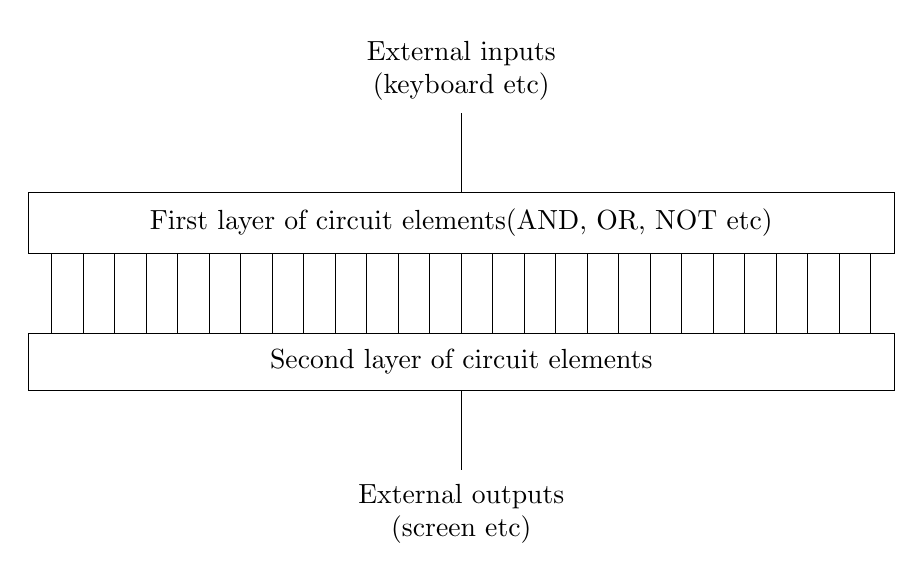
\begin{tikzpicture}

    \foreach \x in {0,...,26}
      \draw (\x * 0.4,0) -- (\x * 0.4, 1);

    \coordinate (t) at (5.2,1);
    \coordinate (b) at (5.2,0);
    \node(layer1) [above,rectangle,draw,minimum width=11cm,inner sep=6pt] at (t) {
      First layer of circuit elements(AND, OR, NOT etc)
    };

    \node(layer2) [below,rectangle,draw,minimum width=11cm,inner sep=6pt] at (b) {
      Second layer of circuit elements
    };
    
    \node(input) [above=of layer1] {
      \begin{tabular}{c}
        External inputs\\
        (keyboard etc)
      \end{tabular}
    };
    
    \node(output) [below=of layer2] {
      \begin{tabular}{c}
        External outputs\\
        (screen etc)
      \end{tabular}
    };

    \coordinate (t0) at (layer1.north);
    \draw (input) to (t0);
    
    \coordinate (b0) at (layer2.south);
    \draw (b0) to (output);

  \end{tikzpicture} 
\end{document}
